% Options for packages loaded elsewhere
\PassOptionsToPackage{unicode}{hyperref}
\PassOptionsToPackage{hyphens}{url}
%
\documentclass[
]{article}
\usepackage{amsmath,amssymb}
\usepackage{iftex}
\ifPDFTeX
  \usepackage[T1]{fontenc}
  \usepackage[utf8]{inputenc}
  \usepackage{textcomp} % provide euro and other symbols
\else % if luatex or xetex
  \usepackage{unicode-math} % this also loads fontspec
  \defaultfontfeatures{Scale=MatchLowercase}
  \defaultfontfeatures[\rmfamily]{Ligatures=TeX,Scale=1}
\fi
\usepackage{lmodern}
\ifPDFTeX\else
  % xetex/luatex font selection
\fi
% Use upquote if available, for straight quotes in verbatim environments
\IfFileExists{upquote.sty}{\usepackage{upquote}}{}
\IfFileExists{microtype.sty}{% use microtype if available
  \usepackage[]{microtype}
  \UseMicrotypeSet[protrusion]{basicmath} % disable protrusion for tt fonts
}{}
\makeatletter
\@ifundefined{KOMAClassName}{% if non-KOMA class
  \IfFileExists{parskip.sty}{%
    \usepackage{parskip}
  }{% else
    \setlength{\parindent}{0pt}
    \setlength{\parskip}{6pt plus 2pt minus 1pt}}
}{% if KOMA class
  \KOMAoptions{parskip=half}}
\makeatother
\usepackage{xcolor}
\usepackage[margin=1in]{geometry}
\usepackage{color}
\usepackage{fancyvrb}
\newcommand{\VerbBar}{|}
\newcommand{\VERB}{\Verb[commandchars=\\\{\}]}
\DefineVerbatimEnvironment{Highlighting}{Verbatim}{commandchars=\\\{\}}
% Add ',fontsize=\small' for more characters per line
\usepackage{framed}
\definecolor{shadecolor}{RGB}{248,248,248}
\newenvironment{Shaded}{\begin{snugshade}}{\end{snugshade}}
\newcommand{\AlertTok}[1]{\textcolor[rgb]{0.94,0.16,0.16}{#1}}
\newcommand{\AnnotationTok}[1]{\textcolor[rgb]{0.56,0.35,0.01}{\textbf{\textit{#1}}}}
\newcommand{\AttributeTok}[1]{\textcolor[rgb]{0.13,0.29,0.53}{#1}}
\newcommand{\BaseNTok}[1]{\textcolor[rgb]{0.00,0.00,0.81}{#1}}
\newcommand{\BuiltInTok}[1]{#1}
\newcommand{\CharTok}[1]{\textcolor[rgb]{0.31,0.60,0.02}{#1}}
\newcommand{\CommentTok}[1]{\textcolor[rgb]{0.56,0.35,0.01}{\textit{#1}}}
\newcommand{\CommentVarTok}[1]{\textcolor[rgb]{0.56,0.35,0.01}{\textbf{\textit{#1}}}}
\newcommand{\ConstantTok}[1]{\textcolor[rgb]{0.56,0.35,0.01}{#1}}
\newcommand{\ControlFlowTok}[1]{\textcolor[rgb]{0.13,0.29,0.53}{\textbf{#1}}}
\newcommand{\DataTypeTok}[1]{\textcolor[rgb]{0.13,0.29,0.53}{#1}}
\newcommand{\DecValTok}[1]{\textcolor[rgb]{0.00,0.00,0.81}{#1}}
\newcommand{\DocumentationTok}[1]{\textcolor[rgb]{0.56,0.35,0.01}{\textbf{\textit{#1}}}}
\newcommand{\ErrorTok}[1]{\textcolor[rgb]{0.64,0.00,0.00}{\textbf{#1}}}
\newcommand{\ExtensionTok}[1]{#1}
\newcommand{\FloatTok}[1]{\textcolor[rgb]{0.00,0.00,0.81}{#1}}
\newcommand{\FunctionTok}[1]{\textcolor[rgb]{0.13,0.29,0.53}{\textbf{#1}}}
\newcommand{\ImportTok}[1]{#1}
\newcommand{\InformationTok}[1]{\textcolor[rgb]{0.56,0.35,0.01}{\textbf{\textit{#1}}}}
\newcommand{\KeywordTok}[1]{\textcolor[rgb]{0.13,0.29,0.53}{\textbf{#1}}}
\newcommand{\NormalTok}[1]{#1}
\newcommand{\OperatorTok}[1]{\textcolor[rgb]{0.81,0.36,0.00}{\textbf{#1}}}
\newcommand{\OtherTok}[1]{\textcolor[rgb]{0.56,0.35,0.01}{#1}}
\newcommand{\PreprocessorTok}[1]{\textcolor[rgb]{0.56,0.35,0.01}{\textit{#1}}}
\newcommand{\RegionMarkerTok}[1]{#1}
\newcommand{\SpecialCharTok}[1]{\textcolor[rgb]{0.81,0.36,0.00}{\textbf{#1}}}
\newcommand{\SpecialStringTok}[1]{\textcolor[rgb]{0.31,0.60,0.02}{#1}}
\newcommand{\StringTok}[1]{\textcolor[rgb]{0.31,0.60,0.02}{#1}}
\newcommand{\VariableTok}[1]{\textcolor[rgb]{0.00,0.00,0.00}{#1}}
\newcommand{\VerbatimStringTok}[1]{\textcolor[rgb]{0.31,0.60,0.02}{#1}}
\newcommand{\WarningTok}[1]{\textcolor[rgb]{0.56,0.35,0.01}{\textbf{\textit{#1}}}}
\usepackage{graphicx}
\makeatletter
\newsavebox\pandoc@box
\newcommand*\pandocbounded[1]{% scales image to fit in text height/width
  \sbox\pandoc@box{#1}%
  \Gscale@div\@tempa{\textheight}{\dimexpr\ht\pandoc@box+\dp\pandoc@box\relax}%
  \Gscale@div\@tempb{\linewidth}{\wd\pandoc@box}%
  \ifdim\@tempb\p@<\@tempa\p@\let\@tempa\@tempb\fi% select the smaller of both
  \ifdim\@tempa\p@<\p@\scalebox{\@tempa}{\usebox\pandoc@box}%
  \else\usebox{\pandoc@box}%
  \fi%
}
% Set default figure placement to htbp
\def\fps@figure{htbp}
\makeatother
\setlength{\emergencystretch}{3em} % prevent overfull lines
\providecommand{\tightlist}{%
  \setlength{\itemsep}{0pt}\setlength{\parskip}{0pt}}
\setcounter{secnumdepth}{-\maxdimen} % remove section numbering
\usepackage{bookmark}
\IfFileExists{xurl.sty}{\usepackage{xurl}}{} % add URL line breaks if available
\urlstyle{same}
\hypersetup{
  pdftitle={Lab 01: Intro to R, Quarto},
  pdfauthor={Maghfira Ramadhani},
  hidelinks,
  pdfcreator={LaTeX via pandoc}}

\title{Lab 01: Intro to R, Quarto}
\author{Maghfira Ramadhani}
\date{2025-09-10}

\begin{document}
\maketitle

\subsection{R Markdown}\label{r-markdown}

This is an R Markdown document. Markdown is a simple formatting syntax
for authoring HTML, PDF, and MS Word documents. For more details on
using R Markdown see \url{http://rmarkdown.rstudio.com}.

When you click the \textbf{Knit} button a document will be generated
that includes both content as well as the output of any embedded R code
chunks within the document. You can embed an R code chunk like this:

\begin{Shaded}
\begin{Highlighting}[]
\FunctionTok{summary}\NormalTok{(cars)}
\end{Highlighting}
\end{Shaded}

\begin{verbatim}
##      speed           dist       
##  Min.   : 4.0   Min.   :  2.00  
##  1st Qu.:12.0   1st Qu.: 26.00  
##  Median :15.0   Median : 36.00  
##  Mean   :15.4   Mean   : 42.98  
##  3rd Qu.:19.0   3rd Qu.: 56.00  
##  Max.   :25.0   Max.   :120.00
\end{verbatim}

\subsection{Including Plots}\label{including-plots}

You can also embed plots, for example:

\pandocbounded{\includegraphics[keepaspectratio]{lab_files/figure-latex/pressure-1.pdf}}

Note that the \texttt{echo\ =\ FALSE} parameter was added to the code
chunk to prevent printing of the R code that generated the plot.

\subsection{Due date}\label{due-date}

This lab is due on \textbf{Monday, September 15 at 11:59pm}. To be
considered on time, the following must be done by the due date:

\begin{itemize}
\tightlist
\item
  Final \texttt{.pdf} file submitted on Gradescope
\end{itemize}

I'd recommend submitting ASAP, as most of today's lab questions will be
able to be done in class, spend your weekend prepping for midterm 1.

\section{Introduction}\label{introduction}

The main goal is to introduce you to R and RStudio. We will use these
throughout the course, both to learn the statistical concepts discussed
in the lecture and to analyze real data and come to informed
conclusions.

R is the name of the programming language itself and RStudio is a
convenient interface.

\subsection{Learning goals}\label{learning-goals}

By the end of the lab, you will\ldots{}

\begin{itemize}
\tightlist
\item
  Be familiar with the workflow using RStudio
\item
  Gain practice writing a reproducible report using Quarto
\item
  Gain practice writing mathematical notation in (LaTeX) in Quarto.
\item
  Perform basic mathematical operations in R.
\item
  Write and read external from and to \texttt{.csv} in R.
\end{itemize}

\section{Getting Started}\label{getting-started}

\subsection{Start a new RStudio
project}\label{start-a-new-rstudio-project}

\begin{itemize}
\tightlist
\item
  Create a new folder on your computer, name it
  \texttt{ECON2250\_Labs\_LastName\_FirstName} (if you are working on
  IAC VLab, you might want to create this folder inside your Dropbox
  folder)
\item
  Go to the Lab 1 module on Canvas, or on the course website, download
  the Quarto markdown file \texttt{lab-01.qmd} to the folder you
  created.
\item
  In RStudio, go to \emph{File} \(\rightarrow\) \emph{New Project}
  \(\rightarrow\) \emph{Existing Directory} \(\rightarrow\) \emph{Select
  your ECON2250 Labs directory} \(\rightarrow\) \emph{Create Project}.
\item
  Now you should see your \texttt{.qmd} file displayed in the
  \emph{Files} pane in RStudio.
\item
  Click \texttt{lab-01.qmd} to open the template Quarto file, rename the
  Author to your full name. This is where you will write up your code
  and narrative for the lab. When you're done with Rstudio, you can
  reopen the project by opening the \texttt{.Rproj} file in the project
  directory.
\end{itemize}

\subsection{R and R Studio}\label{r-and-r-studio}

Below are the components of the RStudio IDE:

\begin{enumerate}
\def\labelenumi{\arabic{enumi}.}
\item
  Source Editor
\item
  Console
\item
  Environment -History - Git
\item
  Files - Plots - Packages - Help - Viewer
\end{enumerate}

\pandocbounded{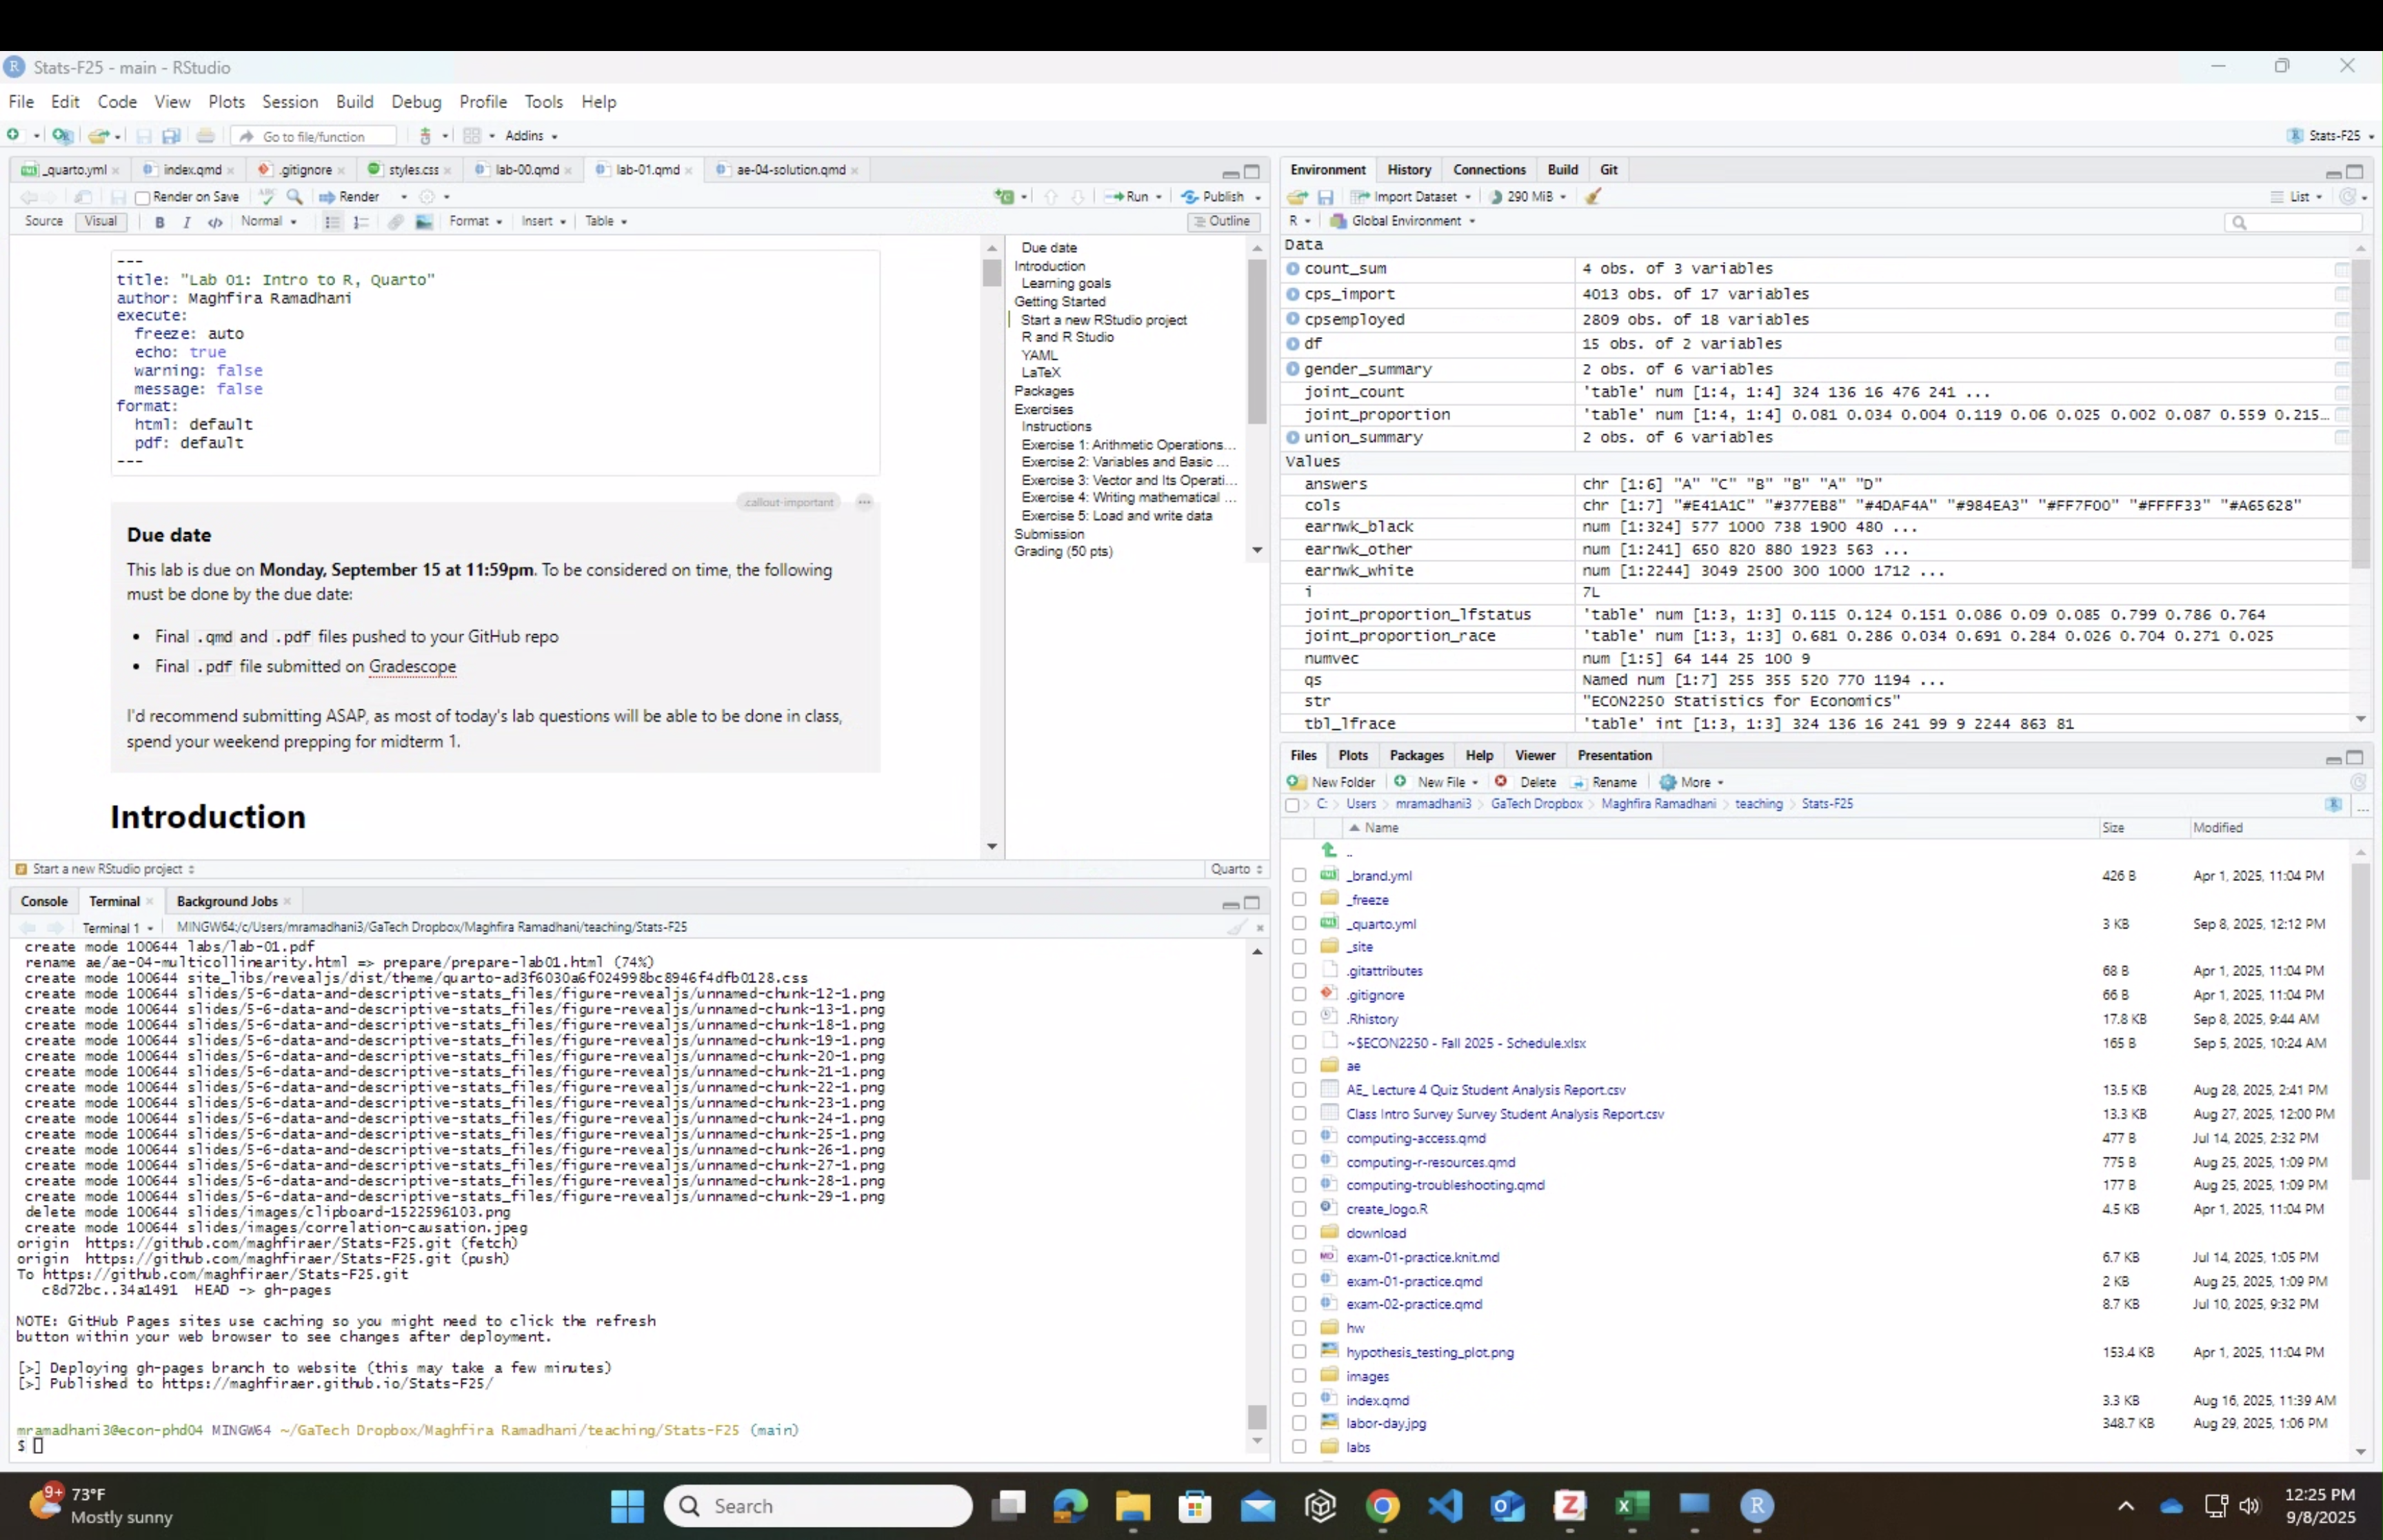
\includegraphics[keepaspectratio]{images/RStudio_pane.png}}

Below are the components of a Quarto (\texttt{.qmd}) file:

\begin{enumerate}
\def\labelenumi{\arabic{enumi}.}
\tightlist
\item
  YAML
\item
  Code chunk
\item
  Narrative
\item
  Rendered output
\end{enumerate}

\pandocbounded{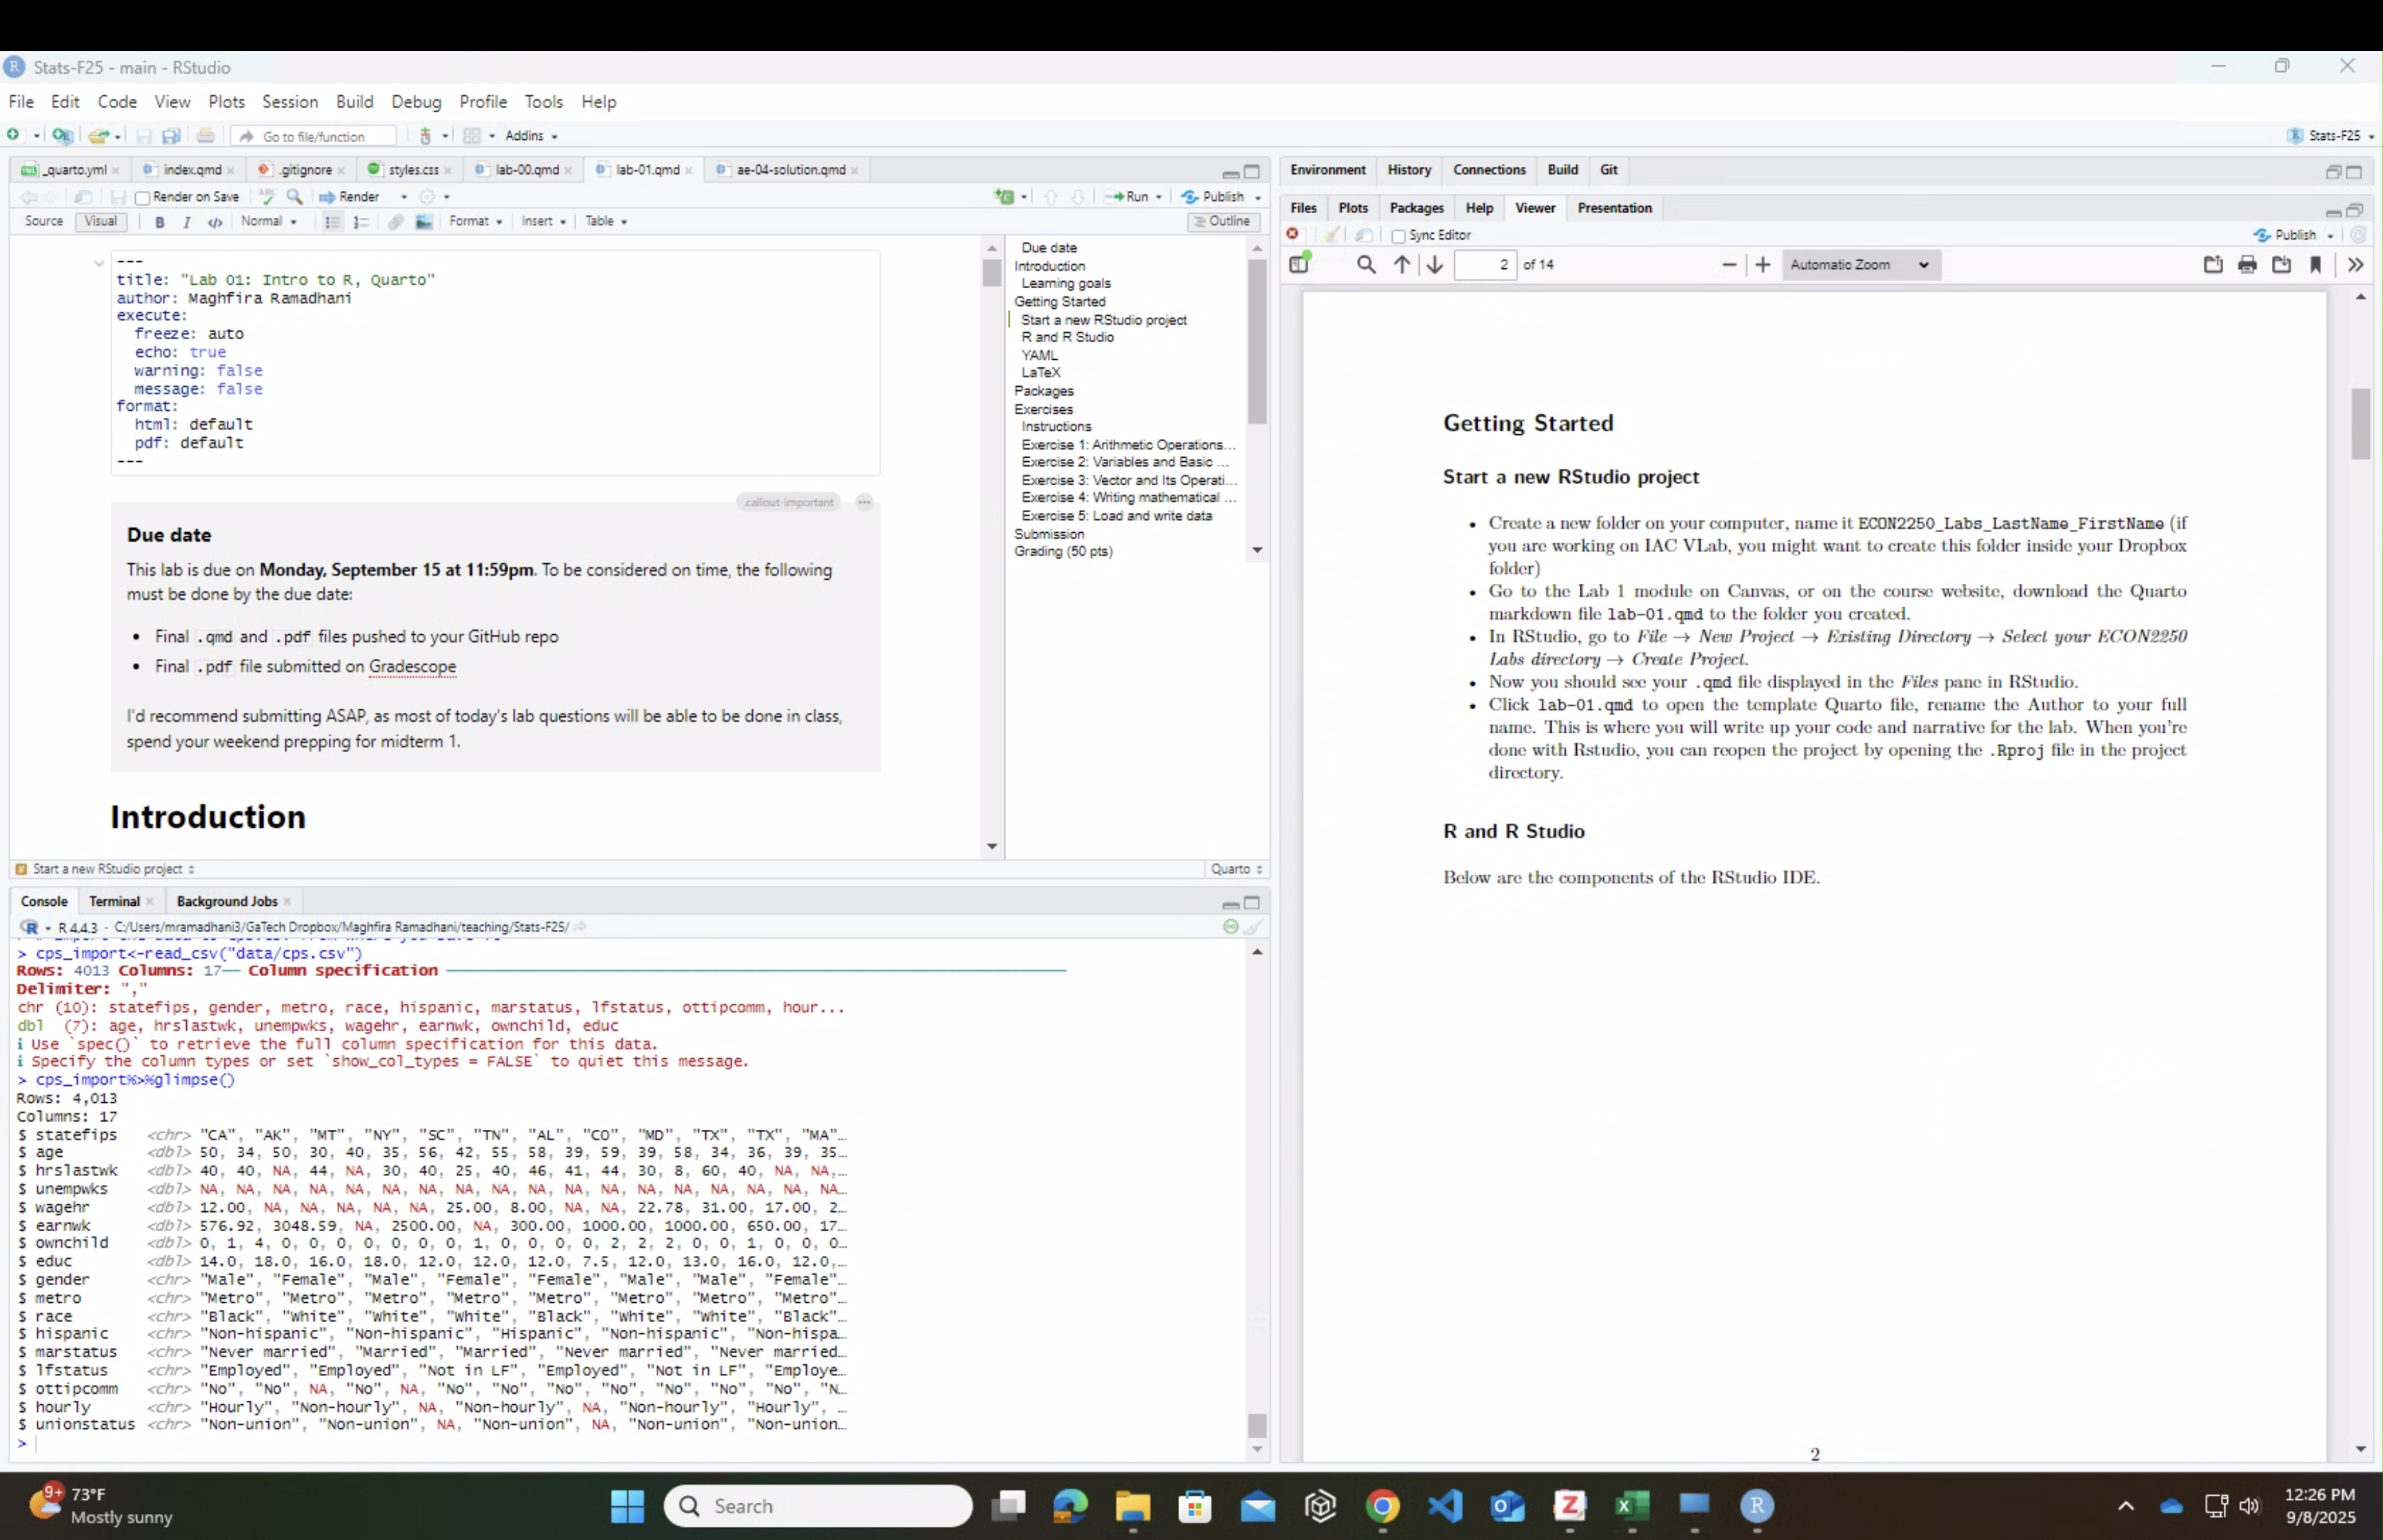
\includegraphics[keepaspectratio]{images/RStudio_render.png}}

\subsection{YAML}\label{yaml}

The top portion of your Quarto file (between the three dashed lines) is
called \textbf{YAML}. It stands for ``YAML Ain't Markup Language''. It
is a human friendly data serialization standard for all programming
languages. All you need to know is that this area is called the YAML (we
will refer to it as such) and that it contains meta information about
your document.

Open the Quarto (.qmd) file in your project, change the author name to
your name, and render the document. Examine the rendered document.

\subsection{LaTeX}\label{latex}

Quarto document uses LaTeX typesetting to write mathematical notation
within the document. We will familiarize ourself with writing
mathematical notation as we goes. Here are some example:

\begin{itemize}
\tightlist
\item
  \texttt{\$x\^{}2+y\^{}2\$} will render as \(x^2+y^2\)
\item
  \texttt{\$\textbackslash{}sum\_\{i=1\}\^{}n\ x\_i=\textbackslash{}overline\{x\}\$}
  will render as \(\sum_{i=1}^n x_i=\overline{x}\)
\end{itemize}

If you're not sure how to write some mathematical notation in LaTeX,
just ask.

\section{Packages}\label{packages}

A package is a collection of programs that someone else has written and
published in public repository (basically a public goods). Package
contain useful command or function so that we don't have to code from
scratch every time. We will need to install the package once before we
can use it using \texttt{install.packages("package1","package2")}. We
also need to load each package before we use them in our code using
\texttt{library(package1)}

We will use the following packages in today's lab.

\begin{Shaded}
\begin{Highlighting}[]
\FunctionTok{library}\NormalTok{(probstats4econ)}
\FunctionTok{library}\NormalTok{(tidyverse)}
\end{Highlighting}
\end{Shaded}

\begin{verbatim}
## -- Attaching core tidyverse packages ------------------------ tidyverse 2.0.0 --
## v dplyr     1.1.4     v readr     2.1.5
## v forcats   1.0.0     v stringr   1.5.2
## v ggplot2   3.5.2     v tibble    3.3.0
## v lubridate 1.9.4     v tidyr     1.3.1
## v purrr     1.1.0     
## -- Conflicts ------------------------------------------ tidyverse_conflicts() --
## x dplyr::filter() masks stats::filter()
## x dplyr::lag()    masks stats::lag()
## i Use the conflicted package (<http://conflicted.r-lib.org/>) to force all conflicts to become errors
\end{verbatim}

\begin{Shaded}
\begin{Highlighting}[]
\FunctionTok{library}\NormalTok{(ggplot2)}
\FunctionTok{library}\NormalTok{(knitr)}
\end{Highlighting}
\end{Shaded}

There's a package manager named \texttt{pacman} that can handle the
package installation for us

\begin{Shaded}
\begin{Highlighting}[]
\CommentTok{\# load and install package if necessary}
\ControlFlowTok{if}\NormalTok{ (}\SpecialCharTok{!}\FunctionTok{require}\NormalTok{(}\StringTok{"pacman"}\NormalTok{)) }\FunctionTok{install.packages}\NormalTok{(}\StringTok{"pacman"}\NormalTok{)}
\end{Highlighting}
\end{Shaded}

\begin{verbatim}
## Loading required package: pacman
\end{verbatim}

\begin{Shaded}
\begin{Highlighting}[]
\NormalTok{pacman}\SpecialCharTok{::}\FunctionTok{p\_load}\NormalTok{(probstats4econ,tidyverse,ggplot2,knitr)}
\end{Highlighting}
\end{Shaded}

\section{Exercises}\label{exercises}

\begin{center}\rule{0.5\linewidth}{0.5pt}\end{center}

\subsection{Instructions}\label{instructions}

Write all code and narrative in your Quarto file. Write all narrative in
complete sentences. Throughout the assignment, you should periodically
\textbf{render} your Quarto document to produce the updated PDF.

Make sure we can read all of your code in your PDF document. This means
you will need to break up long lines of code. One way to help avoid long
lines of code is is start a new line after every pipe
(\texttt{\textbar{}\textgreater{}}) and plus sign (\texttt{+}).

\subsection{Exercise 1: Arithmetic Operations and Mathematical
Functions}\label{exercise-1-arithmetic-operations-and-mathematical-functions}

Here are some mathematical operations in R:

\begin{Shaded}
\begin{Highlighting}[]
\DecValTok{7}\SpecialCharTok{+}\DecValTok{8}
\end{Highlighting}
\end{Shaded}

\begin{verbatim}
## [1] 15
\end{verbatim}

\begin{Shaded}
\begin{Highlighting}[]
\DecValTok{7{-}8}
\end{Highlighting}
\end{Shaded}

\begin{verbatim}
## [1] -1
\end{verbatim}

\begin{Shaded}
\begin{Highlighting}[]
\DecValTok{7}\SpecialCharTok{*}\DecValTok{8}
\end{Highlighting}
\end{Shaded}

\begin{verbatim}
## [1] 56
\end{verbatim}

\begin{Shaded}
\begin{Highlighting}[]
\DecValTok{7}\SpecialCharTok{/}\DecValTok{8}
\end{Highlighting}
\end{Shaded}

\begin{verbatim}
## [1] 0.875
\end{verbatim}

\begin{Shaded}
\begin{Highlighting}[]
\DecValTok{7}\SpecialCharTok{\^{}}\DecValTok{8}
\end{Highlighting}
\end{Shaded}

\begin{verbatim}
## [1] 5764801
\end{verbatim}

\begin{Shaded}
\begin{Highlighting}[]
\DecValTok{1}\SpecialCharTok{/}\DecValTok{3}
\end{Highlighting}
\end{Shaded}

\begin{verbatim}
## [1] 0.3333333
\end{verbatim}

R follows standard mathematical order of operations, which is in the
following order from highest priority:

Parentheses\(\rightarrow\)Exponentiation\(\rightarrow\)Multiplication
and Division\(\rightarrow\)Addition and substraction

Some commonly used mathematical functions are the following:

\begin{itemize}
\tightlist
\item
  Calculates the absolute value \(|x|\): \texttt{abs(x)}
\item
  Calculates the square root \(\sqrt{x}\): \texttt{sqrt(x)}
\item
  Calculates the exponential value \(e^x\): \texttt{exp(x)}
\item
  Calculates the natural logarightm \(\ln{x}\): \texttt{log(x)} or use
  different base \texttt{log(x,base=b)}
\item
  Calculates the factorial \(x!\): \texttt{factorial(x)}
\end{itemize}

Now perform the following exercise:

\begin{enumerate}
\def\labelenumi{\arabic{enumi}.}
\item
  Compute the following calculation using R:

  \begin{enumerate}
  \def\labelenumii{\alph{enumii}.}
  \tightlist
  \item
    Add 9 by 29
  \item
    Multiply 3 by 12
  \item
    Calculates \((1+2^3)^2\).
  \item
    Calculates \(\log_{10} 1000\).
  \end{enumerate}

  Write the code to compute the above quantity below:
\end{enumerate}

\begin{Shaded}
\begin{Highlighting}[]
\CommentTok{\# a}
\DecValTok{9}\SpecialCharTok{+}\DecValTok{29}
\CommentTok{\# b}
\DecValTok{3}\SpecialCharTok{*}\DecValTok{12}
\CommentTok{\# c}
\NormalTok{((}\DecValTok{1}\SpecialCharTok{+}\NormalTok{(}\DecValTok{2}\SpecialCharTok{\^{}}\DecValTok{3}\NormalTok{))}\SpecialCharTok{\^{}}\DecValTok{2}\NormalTok{)}
\CommentTok{\# d}
\FunctionTok{log}\NormalTok{(}\DecValTok{1000}\NormalTok{,}\AttributeTok{base =} \DecValTok{10}\NormalTok{)}
\end{Highlighting}
\end{Shaded}

In this `\texttt{lab-01.qmd\textasciigrave{}} document you'll see that
we already added the code required for the exercise as well as a
sentence where you can fill in the blanks to report the answer. Use this
format for the remaining exercises.

Also note that the code chunk has a label:
\texttt{simple-math-operations}. Labeling your code chunks is not
required, but it is good practice and highly encouraged. Set
\texttt{eval:\ true} if you want the program output to be printed in the
PDF.

\subsection{Exercise 2: Variables and Basic
Operations}\label{exercise-2-variables-and-basic-operations}

Most common data types in R are \texttt{numeric}, \texttt{logical},
\texttt{character}, \texttt{date}, \texttt{factor}.

\begin{Shaded}
\begin{Highlighting}[]
\NormalTok{x }\OtherTok{\textless{}{-}} \DecValTok{1}

\NormalTok{x}

\NormalTok{x}\SpecialCharTok{+}\DecValTok{5}

\NormalTok{x }\OtherTok{\textless{}{-}} \DecValTok{2}\SpecialCharTok{*}\NormalTok{x }\CommentTok{\# Assign new value of x equal 2 times old x}

\NormalTok{x}

\FunctionTok{rm}\NormalTok{(x) }\CommentTok{\# Delete variable x}

\NormalTok{x }\CommentTok{\# As we delete variable x, the program return error won\textquotesingle{}t execute the next line of code}

\NormalTok{y }\OtherTok{\textless{}{-}} \FloatTok{10.5}

\FunctionTok{class}\NormalTok{(y) }\CommentTok{\# Check types of variable y}
\end{Highlighting}
\end{Shaded}

\begin{Shaded}
\begin{Highlighting}[]
\NormalTok{y }\OtherTok{\textless{}{-}} \FloatTok{10.5}

\FunctionTok{class}\NormalTok{(y) }\CommentTok{\# Check types of variable y}
\end{Highlighting}
\end{Shaded}

\begin{verbatim}
## [1] "numeric"
\end{verbatim}

\begin{Shaded}
\begin{Highlighting}[]
\NormalTok{str }\OtherTok{\textless{}{-}} \StringTok{"ECON2250 Statistics for Economics"}
\FunctionTok{class}\NormalTok{(str)}
\end{Highlighting}
\end{Shaded}

\begin{verbatim}
## [1] "character"
\end{verbatim}

Now perform the following exercise:

\begin{enumerate}
\def\labelenumi{\arabic{enumi}.}
\tightlist
\item
  Create variables for the following economic indicators for the United
  States.

  \begin{enumerate}
  \def\labelenumii{\alph{enumii}.}
  \tightlist
  \item
    GDP : 25,000,000,000
  \item
    Inflation Rate: 3.5\%
  \item
    Unemployment Rate: 4.2\%
  \item
    Population: 330 million
  \end{enumerate}
\end{enumerate}

\begin{Shaded}
\begin{Highlighting}[]
\CommentTok{\# GDP}
\NormalTok{GDP }\OtherTok{\textless{}{-}} \StringTok{"25000000000"}
    
\CommentTok{\# Inflation\_Rate}
\NormalTok{Inflation\_Rate }\OtherTok{\textless{}{-}} \StringTok{"0.035"}
    
\CommentTok{\# Unemployment\_Rate}
\NormalTok{Unemployment\_Rate }\OtherTok{\textless{}{-}} \StringTok{"0.042"}

\CommentTok{\# Population}
\NormalTok{Population }\OtherTok{\textless{}{-}} \StringTok{"330000000"}
\end{Highlighting}
\end{Shaded}

\begin{enumerate}
\def\labelenumi{\arabic{enumi}.}
\setcounter{enumi}{1}
\tightlist
\item
  Use these variables to calculate the following:

  \begin{enumerate}
  \def\labelenumii{\alph{enumii}.}
  \tightlist
  \item
    GDP per capita
  \item
    Unemployed individual in the US assuming labor force participation
    of 20\%
  \end{enumerate}
\end{enumerate}

\begin{Shaded}
\begin{Highlighting}[]
\CommentTok{\# GDP\_per\_capita}
\NormalTok{GDP\_per\_capita }\OtherTok{\textless{}{-}}\StringTok{"75.7575757576"}
\NormalTok{GDP\_per\_capita    }

\CommentTok{\# Unemployed\_individuals}
\NormalTok{Unemployed\_individuals }\OtherTok{\textless{}{-}} \StringTok{"2772000"}
\NormalTok{Unemployed\_individuals}
\end{Highlighting}
\end{Shaded}

\begin{enumerate}
\def\labelenumi{\arabic{enumi}.}
\setcounter{enumi}{2}
\tightlist
\item
  Create the following character variables

  \begin{enumerate}
  \def\labelenumii{\alph{enumii}.}
  \tightlist
  \item
    Country: United States
  \item
    Sector: Mixed
  \end{enumerate}
\end{enumerate}

\begin{Shaded}
\begin{Highlighting}[]
\CommentTok{\# Country}
\NormalTok{Country }\OtherTok{\textless{}{-}} \StringTok{"United States"}
\NormalTok{Country}

\CommentTok{\# Sector}
\NormalTok{Sector }\OtherTok{\textless{}{-}} \StringTok{"Mixed"}
\NormalTok{Sector}
\end{Highlighting}
\end{Shaded}

\begin{enumerate}
\def\labelenumi{\arabic{enumi}.}
\setcounter{enumi}{3}
\tightlist
\item
  Check the type of variable for each variable you created.
\end{enumerate}

\begin{Shaded}
\begin{Highlighting}[]
\FunctionTok{class}\NormalTok{(Country)}
\FunctionTok{class}\NormalTok{(Sector)}
\end{Highlighting}
\end{Shaded}

\subsection{Exercise 3: Vector and Its
Operations}\label{exercise-3-vector-and-its-operations}

A vector is a collection of elements of the same data type. The simplest
method to create a vector is with the \texttt{c} function, and we can
determine the length of a vector with the length function as follows:

\begin{Shaded}
\begin{Highlighting}[]
\CommentTok{\# Define vector of numerics}
\NormalTok{numvec }\OtherTok{\textless{}{-}} \FunctionTok{c}\NormalTok{(}\DecValTok{8}\NormalTok{,}\DecValTok{12}\NormalTok{,}\DecValTok{5}\NormalTok{,}\DecValTok{10}\NormalTok{,}\DecValTok{3}\NormalTok{)}
\NormalTok{numvec}
\end{Highlighting}
\end{Shaded}

\begin{verbatim}
## [1]  8 12  5 10  3
\end{verbatim}

\begin{Shaded}
\begin{Highlighting}[]
\NormalTok{numvec}\OtherTok{\textless{}{-}}\NormalTok{numvec}\SpecialCharTok{\^{}}\DecValTok{2}
\NormalTok{numvec}
\end{Highlighting}
\end{Shaded}

\begin{verbatim}
## [1]  64 144  25 100   9
\end{verbatim}

\begin{Shaded}
\begin{Highlighting}[]
\FunctionTok{length}\NormalTok{(numvec)}
\end{Highlighting}
\end{Shaded}

\begin{verbatim}
## [1] 5
\end{verbatim}

\begin{Shaded}
\begin{Highlighting}[]
\CommentTok{\# Define vector of characters}
\NormalTok{answers }\OtherTok{\textless{}{-}} \FunctionTok{c}\NormalTok{(}\StringTok{"A"}\NormalTok{,}\StringTok{"C"}\NormalTok{,}\StringTok{"B"}\NormalTok{,}\StringTok{"B"}\NormalTok{,}\StringTok{"A"}\NormalTok{,}\StringTok{"D"}\NormalTok{)}
\NormalTok{answers}
\end{Highlighting}
\end{Shaded}

\begin{verbatim}
## [1] "A" "C" "B" "B" "A" "D"
\end{verbatim}

\begin{Shaded}
\begin{Highlighting}[]
\FunctionTok{length}\NormalTok{(answers)}
\end{Highlighting}
\end{Shaded}

\begin{verbatim}
## [1] 6
\end{verbatim}

\begin{Shaded}
\begin{Highlighting}[]
\CommentTok{\# Define vector of loficals}
\NormalTok{tfvec }\OtherTok{\textless{}{-}} \FunctionTok{c}\NormalTok{(}\ConstantTok{TRUE}\NormalTok{,}\ConstantTok{FALSE}\NormalTok{,}\ConstantTok{FALSE}\NormalTok{,}\ConstantTok{TRUE}\NormalTok{)}
\NormalTok{tfvec}
\end{Highlighting}
\end{Shaded}

\begin{verbatim}
## [1]  TRUE FALSE FALSE  TRUE
\end{verbatim}

\begin{Shaded}
\begin{Highlighting}[]
\FunctionTok{length}\NormalTok{(tfvec)}
\end{Highlighting}
\end{Shaded}

\begin{verbatim}
## [1] 4
\end{verbatim}

We can also create vector of numerics using \texttt{seq()}, \texttt{:},
or \texttt{rep} functions:

\begin{Shaded}
\begin{Highlighting}[]
\CommentTok{\# Define vector of numerics 1,2,3,...,10}
\FunctionTok{seq}\NormalTok{(}\DecValTok{1}\NormalTok{,}\DecValTok{10}\NormalTok{)}
\end{Highlighting}
\end{Shaded}

\begin{verbatim}
##  [1]  1  2  3  4  5  6  7  8  9 10
\end{verbatim}

\begin{Shaded}
\begin{Highlighting}[]
\FunctionTok{seq}\NormalTok{(}\DecValTok{1}\NormalTok{,}\DecValTok{10}\NormalTok{,}\DecValTok{1}\NormalTok{)}
\end{Highlighting}
\end{Shaded}

\begin{verbatim}
##  [1]  1  2  3  4  5  6  7  8  9 10
\end{verbatim}

\begin{Shaded}
\begin{Highlighting}[]
\DecValTok{1}\SpecialCharTok{:}\DecValTok{10}
\end{Highlighting}
\end{Shaded}

\begin{verbatim}
##  [1]  1  2  3  4  5  6  7  8  9 10
\end{verbatim}

\begin{Shaded}
\begin{Highlighting}[]
\CommentTok{\# Define vector of zeros with length 5}
\FunctionTok{rep}\NormalTok{(}\DecValTok{0}\NormalTok{,}\DecValTok{5}\NormalTok{)}
\end{Highlighting}
\end{Shaded}

\begin{verbatim}
## [1] 0 0 0 0 0
\end{verbatim}

\begin{Shaded}
\begin{Highlighting}[]
\CommentTok{\# We can combine multiple vectors with c()}
\NormalTok{x}\OtherTok{\textless{}{-}}\FunctionTok{c}\NormalTok{(}\DecValTok{1}\SpecialCharTok{:}\DecValTok{10}\NormalTok{,}\FunctionTok{rep}\NormalTok{(}\DecValTok{0}\NormalTok{,}\DecValTok{5}\NormalTok{))}
\NormalTok{x}
\end{Highlighting}
\end{Shaded}

\begin{verbatim}
##  [1]  1  2  3  4  5  6  7  8  9 10  0  0  0  0  0
\end{verbatim}

\begin{Shaded}
\begin{Highlighting}[]
\CommentTok{\# We can acces i{-}th element of a vector}
\NormalTok{x[}\DecValTok{11}\NormalTok{]}
\end{Highlighting}
\end{Shaded}

\begin{verbatim}
## [1] 0
\end{verbatim}

\begin{Shaded}
\begin{Highlighting}[]
\CommentTok{\# We can acces i{-}th to j{-}th element of a vector}
\NormalTok{x[}\DecValTok{1}\SpecialCharTok{:}\DecValTok{5}\NormalTok{]}
\end{Highlighting}
\end{Shaded}

\begin{verbatim}
## [1] 1 2 3 4 5
\end{verbatim}

\begin{Shaded}
\begin{Highlighting}[]
\CommentTok{\# We can acces select element of a vector}
\NormalTok{x[}\FunctionTok{c}\NormalTok{(}\DecValTok{4}\NormalTok{,}\DecValTok{1}\NormalTok{,}\DecValTok{2}\NormalTok{)]}
\end{Highlighting}
\end{Shaded}

\begin{verbatim}
## [1] 4 1 2
\end{verbatim}

Commonly used vector-related functions are \texttt{min(x)},
\texttt{max(x)}, \texttt{sort(x,\ decreasing=FALSE)},
\texttt{unique(x)}, \texttt{sum(x)}, \texttt{mean(x)},
\texttt{cumsum(x)}.

Now perform the following Exercise:

\begin{enumerate}
\def\labelenumi{\arabic{enumi}.}
\tightlist
\item
  Create the following vectors.

  \begin{enumerate}
  \def\labelenumii{\alph{enumii}.}
  \tightlist
  \item
    Quarterly GDP Growth Rates: 1.8\%, 2.0\%, 1.75\%, 1.9\%
  \item
    States: AL, AK, AZ, AR, CA
  \end{enumerate}
\end{enumerate}

\begin{Shaded}
\begin{Highlighting}[]
\CommentTok{\# Define Q\_GDP\_growth\_rate}
\NormalTok{Q\_GDP\_growth\_rate}\OtherTok{\textless{}{-}} \FunctionTok{c}\NormalTok{(}\FloatTok{0.018}\NormalTok{,}\FloatTok{0.02}\NormalTok{,}\FloatTok{0.0175}\NormalTok{,}\FloatTok{0.019}\NormalTok{)}
\NormalTok{Q\_GDP\_growth\_rate}
\FunctionTok{length}\NormalTok{(Q\_GDP\_growth\_rate)}

\CommentTok{\# Define States}
\NormalTok{States}\OtherTok{\textless{}{-}} \FunctionTok{c}\NormalTok{(}\StringTok{"AL"}\NormalTok{,}\StringTok{"AL"}\NormalTok{,}\StringTok{"AZ"}\NormalTok{,}\StringTok{"AR"}\NormalTok{,}\StringTok{"CA"}\NormalTok{)}
\NormalTok{States}
\FunctionTok{length}\NormalTok{(States)}
\end{Highlighting}
\end{Shaded}

\begin{enumerate}
\def\labelenumi{\arabic{enumi}.}
\setcounter{enumi}{1}
\tightlist
\item
  Calculate the following using your vectors.

  \begin{enumerate}
  \def\labelenumii{\alph{enumii}.}
  \tightlist
  \item
    Minimum quarterly GDP growth rate
  \item
    Average of GDP growth rates
  \end{enumerate}
\end{enumerate}

\begin{Shaded}
\begin{Highlighting}[]
\CommentTok{\# Compute the minimum of Q\_GDP\_growth\_rate}
\NormalTok{Min\_Q\_GDP\_growth\_rate}\OtherTok{\textless{}{-}} \FunctionTok{min}\NormalTok{(Q\_GDP\_growth\_rate)}


\CommentTok{\# Compute the average of Q\_GDP\_growth\_rate}
\NormalTok{Mean\_Q\_GDP\_growth\_rate}\OtherTok{\textless{}{-}} \FunctionTok{mean}\NormalTok{(Q\_GDP\_growth\_rate)}
\NormalTok{Mean\_Q\_GDP\_growth\_rate}
\end{Highlighting}
\end{Shaded}

\subsection{Exercise 4: Writing mathematical
notation}\label{exercise-4-writing-mathematical-notation}

Having seen how mathematical notations are written so far, to complete
these exercise, you just need to type the formula for sample covariance
and correlation below:

\textbf{Sample covariance:} \[\frac{1}{n-1}{∑n,i=1​(xi​−xˉ)(yi​−yˉ​)}\]

\textbf{Sample correlation:}
\[\frac{∑n,i=1​(xi​−xˉ)(yi​−yˉ​)}{\sqrt{∑n,i=1​(xi​−xˉ)^2∑n,i=1​(yi​−yˉ​)^2}}\]

\subsection{Exercise 5: Load and write
data}\label{exercise-5-load-and-write-data}

We're going to load the CPS data from the \texttt{probstat4econ}
package.

\begin{Shaded}
\begin{Highlighting}[]
\FunctionTok{library}\NormalTok{(probstats4econ)}
\NormalTok{cps }\SpecialCharTok{\%\textgreater{}\%} \FunctionTok{glimpse}\NormalTok{()}
\end{Highlighting}
\end{Shaded}

\begin{verbatim}
## Rows: 4,013
## Columns: 17
## $ statefips   <fct> CA, AK, MT, NY, SC, TN, AL, CO, MD, TX, TX, MA, AZ, IL, WY~
## $ age         <int> 50, 34, 50, 30, 40, 35, 56, 42, 55, 58, 39, 59, 39, 58, 34~
## $ hrslastwk   <int> 40, 40, NA, 44, NA, 30, 40, 25, 40, 46, 41, 44, 30, 8, 60,~
## $ unempwks    <int> NA, NA, NA, NA, NA, NA, NA, NA, NA, NA, NA, NA, NA, NA, NA~
## $ wagehr      <dbl> 12.00, NA, NA, NA, NA, NA, 25.00, 8.00, NA, NA, 22.78, 31.~
## $ earnwk      <dbl> 576.92, 3048.59, NA, 2500.00, NA, 300.00, 1000.00, 1000.00~
## $ ownchild    <int> 0, 1, 4, 0, 0, 0, 0, 0, 0, 0, 1, 0, 0, 0, 0, 2, 2, 2, 0, 0~
## $ educ        <dbl> 14.0, 18.0, 16.0, 18.0, 12.0, 12.0, 12.0, 7.5, 12.0, 13.0,~
## $ gender      <fct> Male, Female, Male, Female, Female, Male, Male, Female, Fe~
## $ metro       <fct> Metro, Metro, Metro, Metro, Metro, Metro, Metro, Metro, Me~
## $ race        <fct> Black, White, White, White, Black, White, White, Black, Ot~
## $ hispanic    <fct> Non-hispanic, Non-hispanic, Hispanic, Non-hispanic, Non-hi~
## $ marstatus   <fct> Never married, Married, Married, Never married, Never marr~
## $ lfstatus    <fct> Employed, Employed, Not in LF, Employed, Not in LF, Employ~
## $ ottipcomm   <fct> No, No, NA, No, NA, No, No, No, No, No, No, No, No, No, No~
## $ hourly      <fct> Hourly, Non-hourly, NA, Non-hourly, NA, Non-hourly, Hourly~
## $ unionstatus <fct> Non-union, Non-union, NA, Non-union, NA, Non-union, Non-un~
\end{verbatim}

\begin{Shaded}
\begin{Highlighting}[]
\NormalTok{cps }\SpecialCharTok{\%\textgreater{}\%} \FunctionTok{head}\NormalTok{()}
\end{Highlighting}
\end{Shaded}

\begin{verbatim}
##   statefips age hrslastwk unempwks wagehr  earnwk ownchild educ gender metro
## 1        CA  50        40       NA     12  576.92        0   14   Male Metro
## 2        AK  34        40       NA     NA 3048.59        1   18 Female Metro
## 3        MT  50        NA       NA     NA      NA        4   16   Male Metro
## 4        NY  30        44       NA     NA 2500.00        0   18 Female Metro
## 5        SC  40        NA       NA     NA      NA        0   12 Female Metro
## 6        TN  35        30       NA     NA  300.00        0   12   Male Metro
##    race     hispanic     marstatus  lfstatus ottipcomm     hourly unionstatus
## 1 Black Non-hispanic Never married  Employed        No     Hourly   Non-union
## 2 White Non-hispanic       Married  Employed        No Non-hourly   Non-union
## 3 White     Hispanic       Married Not in LF      <NA>       <NA>        <NA>
## 4 White Non-hispanic Never married  Employed        No Non-hourly   Non-union
## 5 Black Non-hispanic Never married Not in LF      <NA>       <NA>        <NA>
## 6 White Non-hispanic      Divorced  Employed        No Non-hourly   Non-union
\end{verbatim}

Now we write the cps data locally to our computer

\begin{Shaded}
\begin{Highlighting}[]
\CommentTok{\# Export the data to cps.csv in our project folder, }
\CommentTok{\# you can also write it into a subfolder "data"}
\FunctionTok{write\_csv}\NormalTok{(cps,}\StringTok{"cps.csv"}\NormalTok{)}
\end{Highlighting}
\end{Shaded}

Now to complete this exercise, you have to load the \texttt{.csv} and
show the data below:

\begin{Shaded}
\begin{Highlighting}[]
\CommentTok{\# Import the data to cps.csv from where you save it}
\NormalTok{cps\_import }\OtherTok{\textless{}{-}} \FunctionTok{read\_csv}\NormalTok{(}\StringTok{"cps.csv"}\NormalTok{)}

\CommentTok{\# Show a glimpse of the data here}
\FunctionTok{glimpse}\NormalTok{(cps\_import)}
\end{Highlighting}
\end{Shaded}

\section{Submission}\label{submission}

You will submit the PDF documents and Quarto markdown files for labs,
homework, and exams in to Gradescope as part of your final submission.

Remember -- you must turn in a PDF file to the Gradescope page before
the submission deadline for full credit.

Instructions to combine PDFs:

\begin{itemize}
\item
  Preview (Mac):
  \href{https://support.apple.com/guide/preview/combine-pdfs-prvw43696/mac}{support.apple.com/guide/preview/combine-pdfs-prvw43696/mac}
\item
  Adobe (Mac or PC):
  \href{https://helpx.adobe.com/acrobat/using/merging-files-single-pdf.html}{helpx.adobe.com/acrobat/using/merging-files-single-pdf.html}
\end{itemize}

To submit your assignment:

\begin{itemize}
\item
  Access Gradescope
\item
  Click on the assignment, and you'll be prompted to submit it.
\item
  Mark the pages associated with each exercise. All of the pages of your
  lab should be associated with at least one question (i.e., should be
  ``checked'').
\item
  Select the first page of your .PDF submission to be associated with
  the \emph{``Workflow \& formatting''} section.
\end{itemize}

\section{Grading (50 pts)}\label{grading-50-pts}

\textbf{This lab will be graded for completion, with each exercise worth
10 points. For example, if you complete all 5 exercises, you will
receive a score of 50/50 for Lab 01. If you complete 3 exercises, you
will receive a score of 30/50.}

You will receive feedback on Lab 01, particularly if you have an error
or an incomplete submission, as this is just an introduction to R.

You will receive feedback about ``Workflow \& formatting'' for this lab,
so you know what to expect for grading in future assignments. It will
not count towards the grade in Lab 01.

\end{document}
